\section{Algorithmic details}
The section provides algorithmic details that were not covered in the
main paper.

\subsection{Pre-processing}

Points cloud acquired by multiple depth sensors are generally corrupted
by mirrors, windows, reflective objects, and calibration errors, which
may affect the quality of reconstruction. Therefore, we first remove
noisy 3D points by the following two filters.

\mysubsubsection{Intensity-based filtering}
%for window and reflective objects}
Most depth sensors emit the infrared
light and record the pixel-wise intensity of the reflected light. At the
presence of windows or reflective objects, corresponding intensity
values become low. Therefore, we remove points if the intensity values
are less than $\mu_I - \sigma_I$, where $\mu_I$ and $\sigma_I$ are the
mean and the standard deviation of the intensities in that image.

\mysubsubsection{Connected-component filtering} The intensity thresholding
is not effective against the mirrors, however these 3D points tend to be
highly isolated. We compute the binary
mask in exactly the same way as the computation of $\Psi$ in the room
segmentation, but this time, based only on one panorama depth image. We
simply keep the largest connected component and discard 3D points that
project outside. This filtering is conducted for each panorama depth image.
% On the other hand we observed that mirrored points cloud could be
% detected by looking at the 2-D projection of the point cloud. Since the
% vertical viewing angle of a standard depth sensor is relatively small
% (\eg, 57 degrees for Microsoft Kinect), the floor points between mirror
% surface and mirrored points are missing (See
% \Fref{fig:noiseremoval}). Based on the observation, we project the all
% 2-D points onto the Manhattan $X-Y$ plane, and remove the significantly
% isolated points on the 2-D plane.
%
This criteria may not completely remove the mirror points, but
is enough for our algorithm to suppress further noise in the
reconstruction process.


% \begin{figure}[!t]
% 	\begin{center}
% 		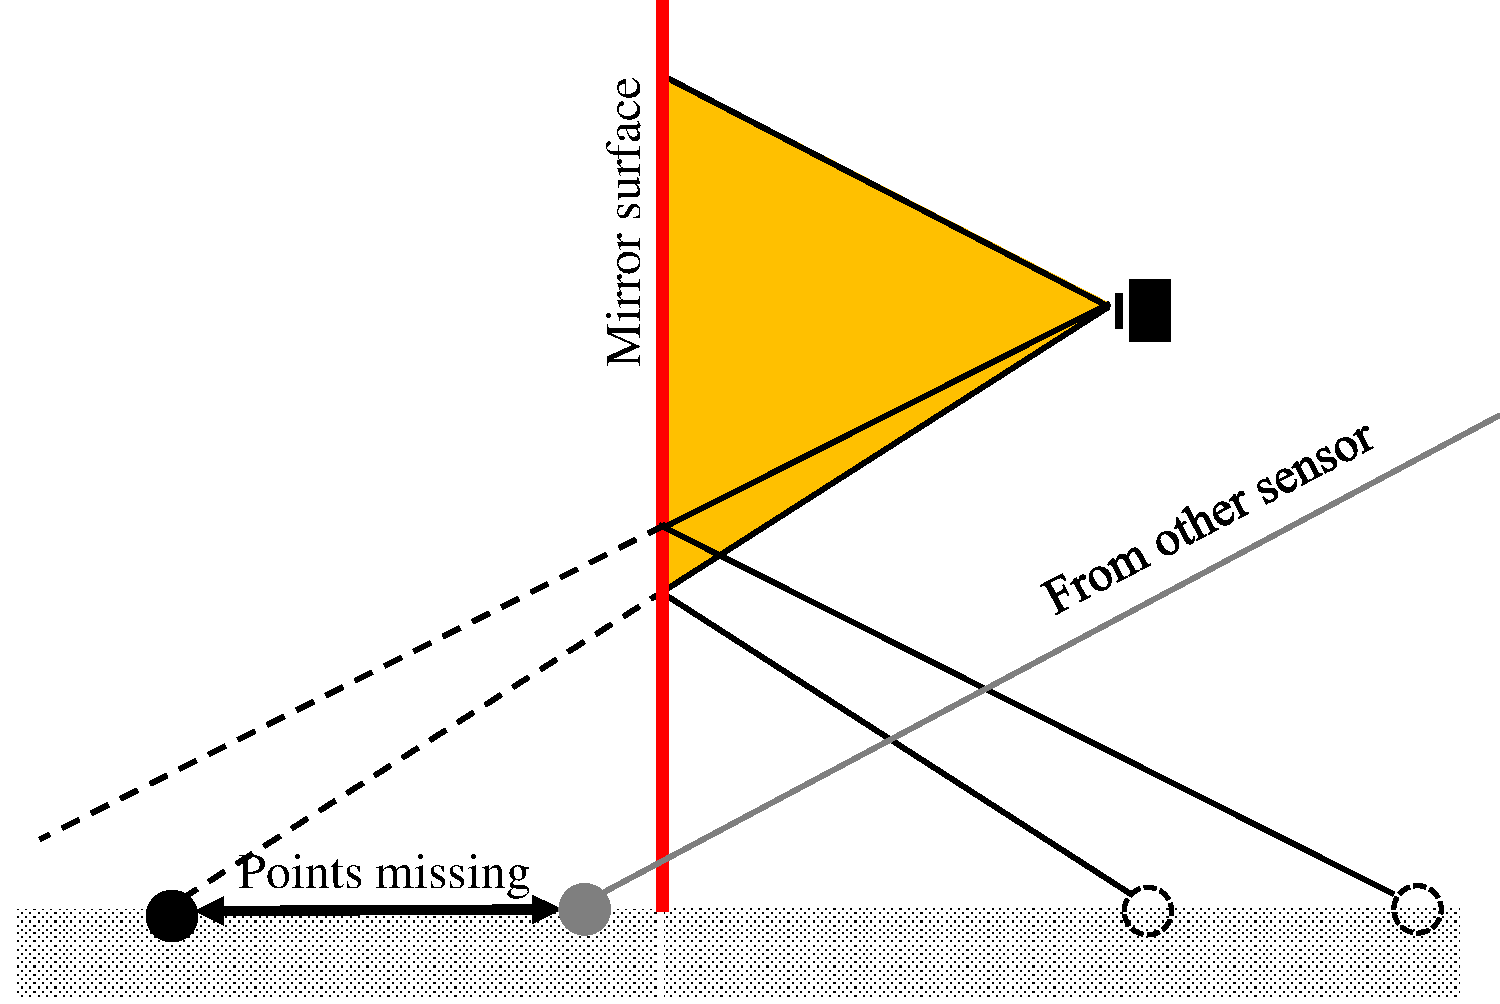
\includegraphics[width=85mm]{../figures/noiseremoval.pdf}
% 	\end{center}
% 	\vspace{-0.2cm}
% 	\caption{When the point is reflected on the mirror, generally the missing region is observed between mirror surface and the mirrored points.}  \label{fig:noiseremoval}
% 	\vspace{-0.25cm}
% \end{figure}


\subsection{Room reconstruction}
The room reconstruction algorithm is based on the previous
work~\cite{floorplan_14}, while we make an adjustment to the {\em core
free-space region} extraction algorithm. The core free-space is computed
as the space with very high free-space evidence, where the room boundary
should not pass through. This caused a problem in our setting. Our
input comes from a depth sensor, while their input is an MVS
point-cloud. A depth sensor generates very strong outliers near the
windows, and their core free-space region often crosses walls through the
windows.

Our approach is to restrict the core free-space region to be an axis
aligned rectangle. More specifically, we find the axis-aligned rectangle
that fits inside the domain $\Psi$ and minimizes the following objective
function:
\begin{eqnarray*}
 max(H, W) + \eta H W,
\end{eqnarray*}
where $H$ and $W$ denote the width and height of the rectangle, and
$\eta=0.001$ is used in our experiments.  This objective has an effect
to maximize the rectangle while keeping its aspect ratio close to 1. We
find the solution via the exhaustive search.


% Here we describe the details of our room reconstruction grammer that we
% omitted due to the space limit. The major framework of the algorithm is
% same with the previous work~\cite{Cabral2014}, that contains (a)
% core-freespace generation, (b) start-end line extraction, (c) path
% optimization. However, we take slightly different strategies since the
% original algorithm is optimized for single room room, while we tackle
% the building scale reconstruction.

% \mysubsubsection{Initialization} The input of the
% algorithm~\cite{Cabral2014} is wall evidence and free-space evidence,
% where wall evidence is the point evidence generated from the points
% whose normal is either of ${X,-X,Y,-Y}$. Here we define wall-evidence
% and free-space evidence {\it independently} for each room
% reconstruction. First, we divide frees-space into regions based on the
% structured graph. While our room node does not always cover the entire
% region as shown in third row of Fig. 2 in the main manuscript, we
% spatially propagate labels so that every pixel in the fees-space
% evidence has a label that corresponds to the room index on the
% graph. And then we compute the wall and free-space evidence where pixels
% in the region of the target room.  (I will add fig later). This per-room
% evidences make the algorithm quite robust and computation of the path
% much more efficient.


% The core free-space region as a high free-space evidence as defined
% in~\cite{Cabral2014} is problematic for our condition since the
% frees-space generally brides different room (even though we define the
% local evidence) and per-room reconstruction becomes impossible.

% Therefore, we instead compute the core free-space by solving following
% optimization problem,
% \begin{equation}
% \min_{\Omega \in RectSet} max(H_{\Omega}, W_{\Omega}) + \gamma H_{\Omega}W_{\Omega}.
% \end{equation}
% where ${RectSet}$ is a collection of rectangles that are completely
% included in the non-zero regions of local free-space evidence and
% $H_\Omega$ and $W_\Omega$ are height and width of a rectangle
% proposal. This equation maximizes the size of core-freespace
% region($\Omega$) while preventing the shape of the evidence from being
% too elongated. This equation quantifies the reasonable observation that
% the room shape is generally convex except for the door part and details
% on the wall such as windows.

% \mysubsubsection{Shortest path reconstruction} Given three information
% (a) the local evidence, (b) the core free-space, and (c) the start-end
% line (in the same manner with~\cite{Cabral2014}), then we reconstruct
% the shortest path that minimize the total edge.

% While \cite{Cabral2014} prevents the path go through the high free-space
% evidence by the hard constraint (core free-space), we instead avoid the
% path to go thorough the high free-space evidence as a penalty in the
% edge cost:
% \begin{eqnarray}
% e_{\rho} = \frac{1}{1+\beta}\sum_{k=1}^{|\rho|}{\left(1-P_W(c_k)+ \beta(c_k) F(c_k)\right)}\nonumber\\
% +\omega,\label{eq:edgecost}
% \end{eqnarray}
% where $c_k$ is a cell that is included in on edge $\rho$. $\omega$ is a
% constant mode-complexity penalty, which biases our solution towards
% paths with less edges ($\omega = 7$ in our experiments). $\beta$ is a
% weight that balances the contribution the free-space evidence and wall
% evidence ($\beta(c_k) = 1$ if $P_W(c_k) = 0$ and $\beta(c_k) = 1.5$ if
% $P_W(c_k) > 0$ in our experiments. We vary $\beta$ for strongly
% penalizing the path that go through the empty cell).

% The optimization is achieved in the same manner with~\cite{Cabral2014}
% and the resultant shortest path is composed of the multiple edges:
% $\rho_1, \rho_2, \cdots, \rho_m$, we define them as the |{\it wall
% elements} in our structured graph.

\subsection{Wall/ceiling detail reconstruction}

% \begin{figure}[!t]
% 	\begin{center}
% 		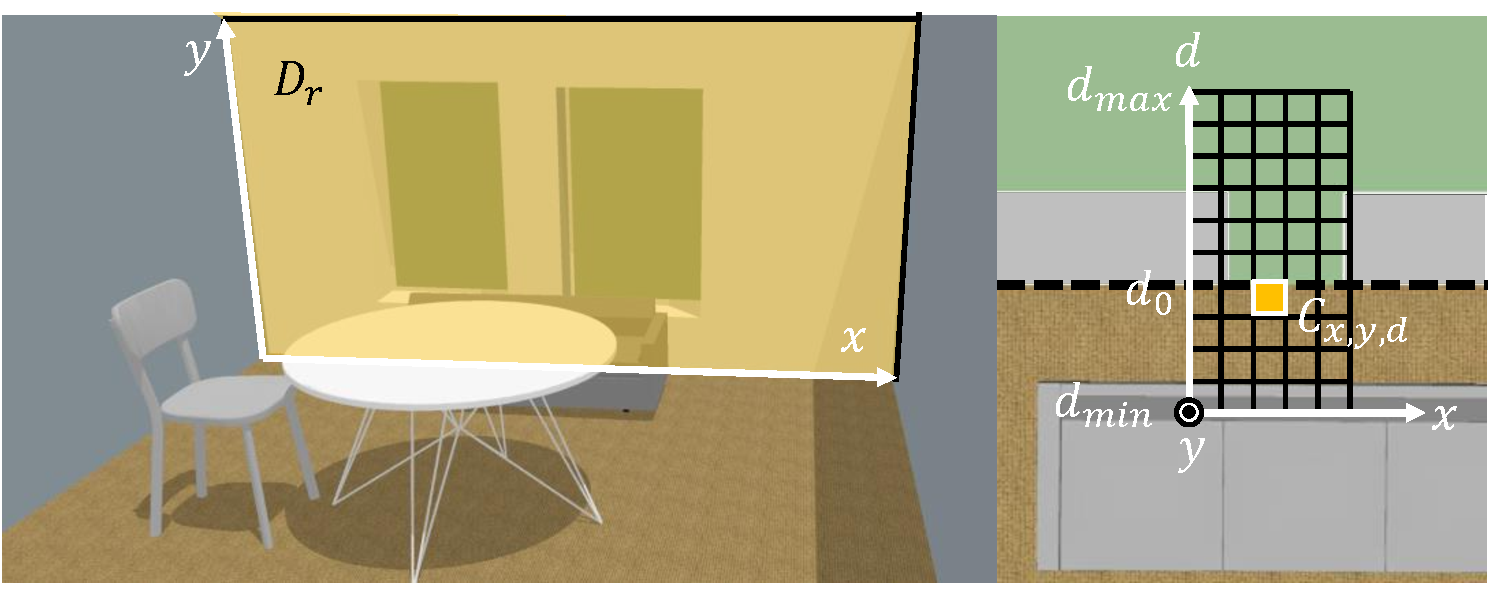
\includegraphics[width=85mm]{../figures/detailreconstruction.pdf}
% 	\end{center}
% 	\vspace{-0.2cm}
% 	\caption{Given a target wall, we construct the costvolume aligned with the Manhattan-World directions. The offset-map is then computed on the $x$-$y$ plane by aggregating the cost via MRF optimization. }  \label{fig:detailreconstruction}
% 	\vspace{-0.25cm}
% \end{figure}
% In this section, we describe the initialization of the offset map
% ($D_r$) in our main manuscript.

% We firstly define the cost-volume that is parallel to the Manhattan
% directions whose inbound and outbound range from the base plane is
% $d_{min}$ and $d_{max}$, respectively (See
% \Fref{fig:detailreconstruction}).

The initial offset-map in the wall/ceiling detail reconstruction is
obtained by a simple 2D MRF with unary and pairwise terms:
\begin{eqnarray*}
 E = \sum_p E_d(d_p) + \lambda \sum_{\{p,q\} \in \mathcal{N}} E_s(d_p, d_q).
\end{eqnarray*}
$p$ and $q$ denote pixels, while $d_p$ is the estimated offset-value at
pixel p.  The pairwise term $E_s$ follows a $Potts$ model where $\lambda
= 0.01$ is used in our experiments. The unary term $E_d$ is defined
as
\begin{equation*}
E_d(d_p) = -P(p, d_p)\left(\sum_{d=d_p^{min}}^{d_p} F(p, d)\right). \label{eq:costdetail}
\end{equation*}
$P(p, d_p)$ and $F(p, d_p)$ denote the point and free-space evidence at
pixel $p$ and offset $d_p$, respectively. Intuitively, the cost becomes
smaller if the point evidence and the accumulation of the free-space
evidence are large. The valid depth range of a pixel $[d_p^{min},
d_p^{max}]$ is computed from the domain $\Psi$ for the room segmentation
in the top-down view. More concretely, we simply cast rays in the two
opposing directions orthogonal to the wall, and obtain the first
intersection with the boundary of $\Psi$ each. Finally, we get the
intersection with the range $[-2\mbox{m}, 2\mbox{m}]$ to avoid unnecessarily large
search space.



% where $P$ and $F$ are the point/free-space evidence, and $x$, $y$ and $d$ are the indices of a cell with regard to wall ($x-y$) and depth ($d$) directions, respectively. 

% Intuitively, if we cast a ray from $d=d_{min}$ to the outgoing direction
% that is perpendicular to the wall, the cost is minimized at the out-most
% intersection to the surface. However, the input point cloud is often
% sparse near the wall and it happens that the ray from the viewpoint does
% not intersect with any points (\ie, the cost for any off-set values is
% zero). For tackling this issue, we simply propagate the information from
% the neighborhood pixels by solving the MRF-optimization problem as
% \begin{equation}
% D_0 = \argmin_{\textbf{d}}{\sum_{p}Cost(p,l) + \lambda \sum_p{\sum_{q\in N(p)}}{Potts(l_p, l_q)}},
% \end{equation}
% where $p$ is an index on the $x-y$ plane, $Potts$ is the potts penalty
% that gives zero if two labels are same and otherwise one ($\lambda =
% 0.01$ in our experiment). Then, the offset-map is used as an initial
% values of $D_r$ as we have already mentioned in the main manuscript.


